%!TEX root = ./main.tex


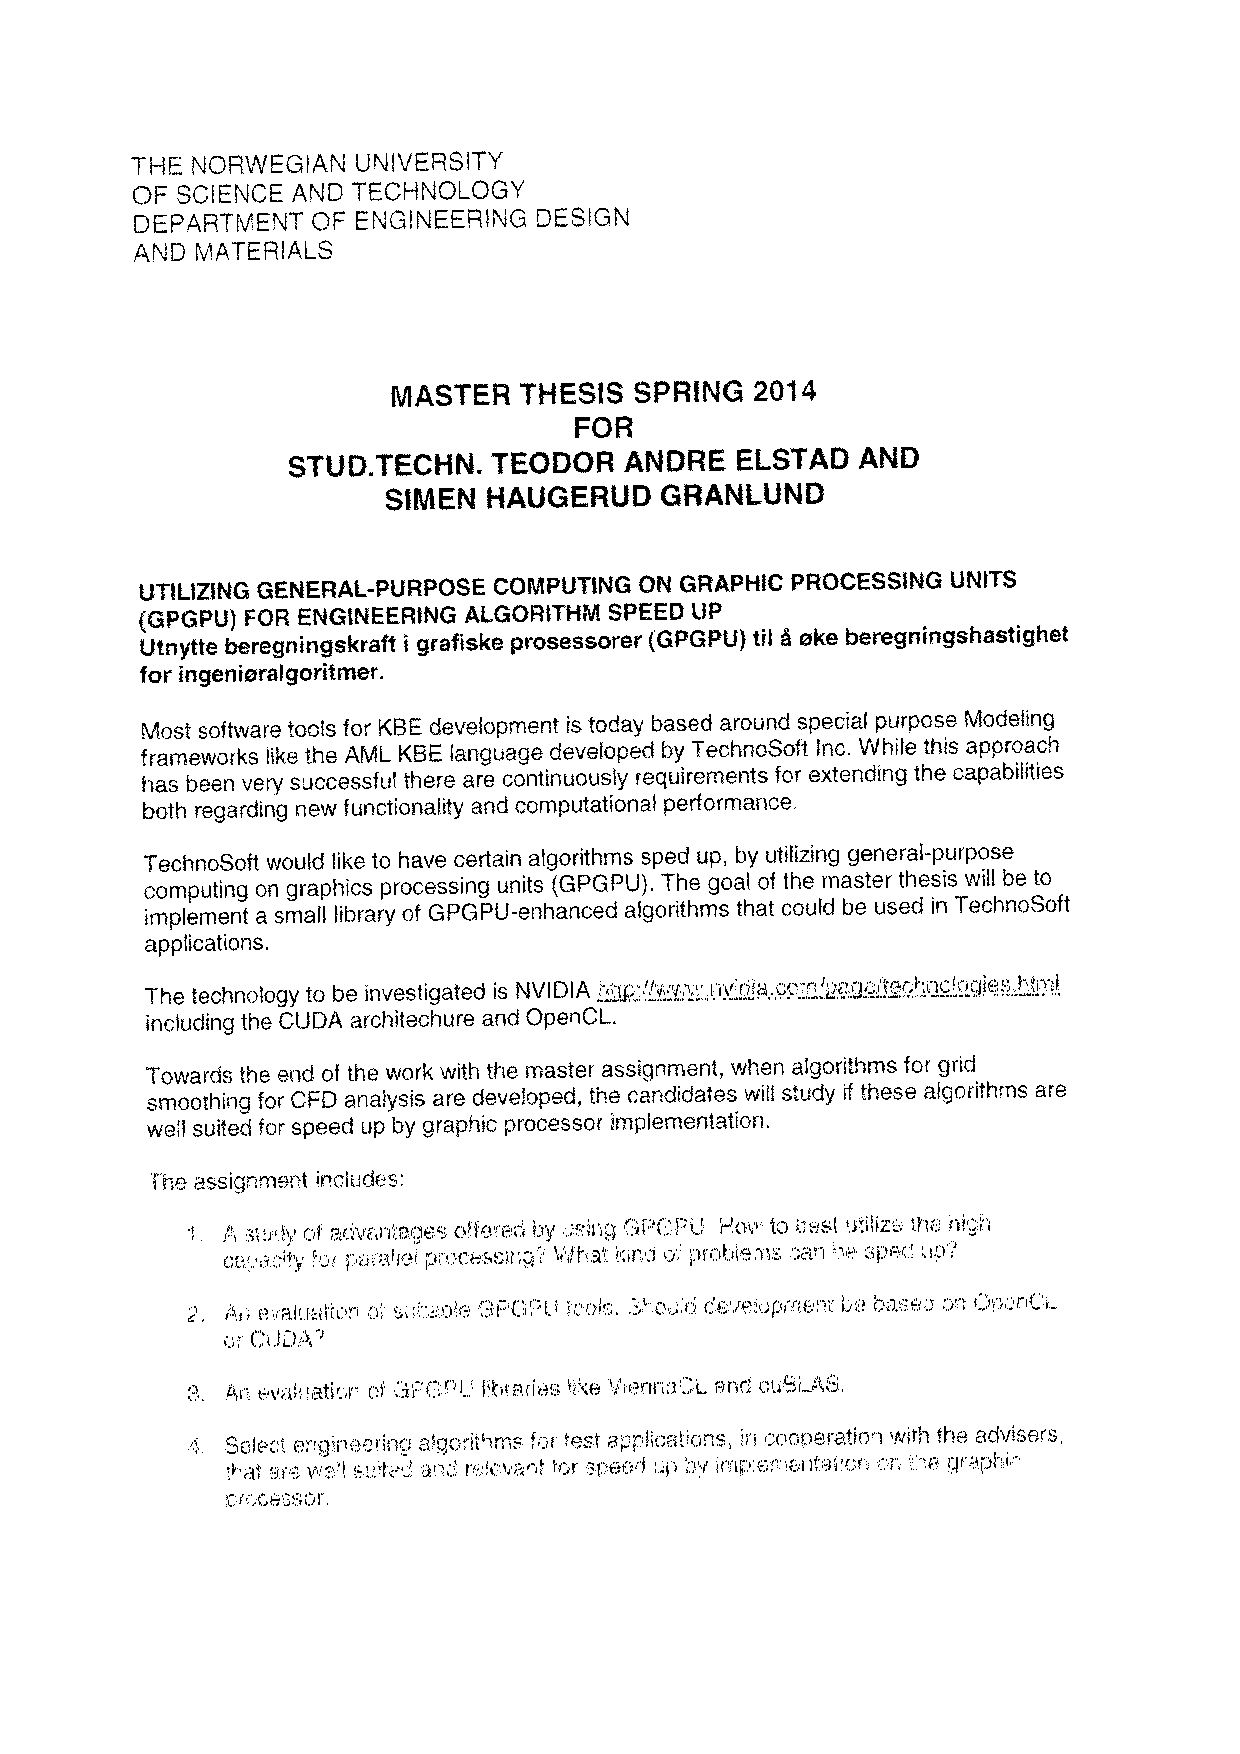
\includepdf[fitpaper=true, pages={1,2}, scale=1, noautoscale]{../gfx/assignment.pdf}
\newpage

% \section*{Assignment}

% \paragraph{} % (fold)
% Most software tools for KBE development is today based around special purpose Modeling frameworks like the AML KBE language developed by TechnoSoft Inc. While this approach has been very successful there are continuously requirements for extending the capabilities both regarding new functionality and computational performance. TechnoSoft would like to have certain algorithms sped up, by utilizing general-purpose computing on graphics processing units (GPGPU). The goal of the master thesis will be to implement a small library of GPGPU-enhanced algorithms that could be used in TechnoSoft applications. The technology to be investigated is NVIDIA http://www.nvidia.com/page/technologies.html including the CUDA architechure and OpenCL. Towards the end of the work with the master assignment, when algorithms for grid smoothing for CFD analysis are developed, the candidates will study if these algorithms are well suited for speed up by graphic processor implementation.
% % paragraph (end)

% \paragraph{The assignment includes:} % (fold)
% \label{par:the_assignment_includes_}

% % paragraph the_assignment_includes_ (end)
% \begin{itemize}
% \item A study of advantages offered by using GPGPU. How to best utilize the high capacity for parallel processing? What kind of problems can be sped up?
% \item An evaluation of suitable GPGPU tools. Should development be based on OpenCL or CUDA?
% \item An evaluation of GPGPU libraries like ViennaCL and cuBLAS.
% \item Select engineering algorithms for test applications, in cooperation with the advisers, that are well suited and relevant for speed up by implementation on the graphic processor.
% \item Extensive performance testing of different implementations on different problem sizes and hardware. Are we getting good speed up on real life problems and hardware, or is the overhead associated with parallel computing hampering performance?
% \end{itemize}
